\documentclass[prl,nofootinbib,twocolumn,floatfix,showpacs]{revtex4}
%\documentclass[manuscript]{revtex4}
\usepackage{graphicx}
\usepackage{amsmath}
\usepackage{amssymb}

\begin{document}
\title{Anharmonicity and mode-coupling in a fluctuating protein}

\author{}
%\email{akabakcioglu@ku.edu.tr}
\affiliation{Ko\c c University, Sar\i yer 34450 \. Istanbul, Turkey}

\date{\today }

\begin{abstract}
%%   I review the expansion of a multivariate probability distribution in terms
%%   of tensor Hermite polynomials and then discuss how the anharmonic terms of
%%   the form $x_1^\alpha x_2^\beta$ can be calculated in terms of the
%%   expectation values $\langle x_1^ix_2^j\rangle$. The result reduces the
%%   problem to calculation of Hermite polynomials $H_n(q)$ in one dimension, the
%%   coefficients of which one can write down in closed form. The method can be
%%   generalized to include three-point correlations $\langle x_1^ix_2^jx_3^k\rangle$.
\end{abstract}

\pacs{}

\maketitle

Residue fluctuations of a protein around its native state reveal
information that bridges the molecule's structural and functional
properties.  At the lowest order, these fluctuations can be treated as
a collection of independent harmonic modes, yielding ``Elastic Network
Models''~\cite{ENM}. However, it was recently shown that the slowest
oscillatory modes of a protein are strongly
anharmonic~\cite{Yogurtcu}, in contrast with the assumption underlying
ENMs. The coupling between different modes is another aspect of
protein dynamics that is believed to be relevant for the
information/energy transfer between different parts of the
molecule~\cite{mode_coupling_ref} and not captured by the harmonicity
assumption. We here develop a general framework for the residue
fluctuations that simultaneously incorporates both anharmonicity and
mode-coupling in a unified formalism. We show that both deviations
from the pure Gaussian model are important for modeling the
multidimensional energy landscape in the vicinity of the native state,
even at physiological conditions where fluctuations are relatively
small. (at what temperature is the MD?)


Sampling the time evolution of a protein by using molecular dynamics
reveals a multivariate probability distribution function $f({\bf\Delta
  R})$ for the deviations of atoms (assume there are $N$ of them) from
equilibrium coordinates, i.e. $\Delta R_i = R_i - R_i^{eq}$,
$i=1,\dots,3N$. We here adopt a coarse-grained representation of this
p.d.f., where only $C_\alpha$ atoms are considered; i.e., $N$ is the
number of residues. Since the deviations from the free energy minimum
should be harmonic for sufficiently small amplitudes, Hermite
polynomials, which have a Gaussian kernel, constitute a natural basis
for representing $f({\bf\Delta R})$. First, following
Ref.~\cite{Yogurtcu}, we perform the transformation
\begin{eqnarray}
\label{transformation}
{\bf \Delta r} &=& \langle {\bf\Delta R \Delta R}^T\rangle ^{-1/2} {\bf
  \Delta R}
\end{eqnarray}
which diagonalizes the covariance matrix and would give the normal
modes of the protein if fluctuations were harmonic. Otherwise, the
distribution function for $\{\Delta r\}$ in its most general form, can
be expressed as~\cite{Flory}
\begin{eqnarray}
f({\bf\Delta r}) &=& \frac{1}{\sqrt{(2\pi)^{3N}}} e^{
    -{\sum_{i=1}^{3N} \Delta r_i^2}/2} \bigg[ 1 +  \sum_{\nu=3}^\infty
 {\bf C_\nu}\cdot {\bf H}_\nu({\bf \Delta r}) \bigg] \nonumber \\
&& \label{hermite_expansion}
\end{eqnarray}
where ${\bf C}_\nu$ (constant) and ${\bf H}_\nu$ (derived below) are
tensors of rank $\nu$, and the dot product refers to
$\sum_{ij..k}\,C_\nu^{ij..k}\,H_\nu^{ij..k}$.  The fluctuations in
this ``normal'' basis are meanless, i.e., $\langle {\Delta r_i}\rangle
= 0$, and decoupled at the lowest (second) order, i.e., $ \langle {
  \Delta r_i^T \Delta r_j}\rangle = \delta_{ij}$. $C_\nu = 0,\ \forall \nu$
corresponds to a purely harmonic model.

As a reminder to the reader, tensor Hermite polynomials can be
obtained by successive differentiation using Rodrigues' formula:
\begin{eqnarray}
\label{Rodrigues}
H_{\nu}^{ij..k}({\bf \Delta r}) &=& \frac{(-1)^\nu}{g({\bf
    \Delta r})}\,{\bf\nabla}^{ij..k}\,g({\bf \Delta r})\ .
\end{eqnarray}
Above, $g({\bf x}) = (2\pi)^{3N/2}\exp(-{\bf x}^2/2)$ is the
multi-dimen{\-}sional Gaussian distribution and ${\bf \nabla}^{ij..k} =
\nabla^i\nabla^j\,..\,\nabla^k$ is the gradient tensor with
$\nabla^i \equiv \partial/\partial x_i$. Explicitly,
\begin{eqnarray}
{\bf H}^{ij}_2({\bf \Delta r}) &=& \Delta r_i\Delta r_j - \delta_{ij} \nonumber \\
{\bf H}^{ijk}_3({\bf \Delta r}) &=& \Delta r_i\Delta r_j\Delta r_k - \delta_{ij}\Delta r_k- \delta_{jk}\Delta r_i- \delta_{ki}\Delta r_j \nonumber \\
& \cdots &
\end{eqnarray}
where $i$, $j$, $k$ run over the components of the vector ${\bf\Delta
  r}$. Higher order Hermite polynomials can be obtained by summing all
possible $0,1,.., \lfloor\frac{\nu}{2}\rfloor$ pairwise
contractions ($\delta_{ij}$s)  of $\Delta r_i\Delta r_j\,..\,\Delta r_k$, a minus sign
accompanying the terms obtained by an odd number of
contractions. Diagonal elements of ${\bf H}_\nu$ (corresponding to a
scalar $\Delta r$) are the usual Hermite polynomials
\begin{eqnarray}
H_\nu(\Delta r) &=& \sum_{m=0}^{\nu/2} (-1)^m\, {\nu \choose 2m} \,m!!\,\Delta r^{\nu-2m}
\label{hermite_anal}
\end{eqnarray}
where $m!!\equiv \frac{(2m)!}{2^m m!} = (2m-1)(2m-3)\cdots 3\cdot
1$, and the combinatorial expression counts the number of $m$ pairwise
contractions of $\nu$ variables.


The orthogonality condition for the Hermite tensor polynomials,
\begin{eqnarray}
\int_{-\infty}^{\infty}{\bf dx}\, \big[{\bf A}_\nu\cdot {\bf H}_\nu({\bf x})\big] {\bf
  H}_\mu({\bf x})e^{-{\bf x}^2/2} &=& \begin{cases}{\bf A}_\nu\nu !\ , & \nu=\mu
  \\ 0\ , & \nu\neq\mu \end{cases} \nonumber \\
&&\label{orthogonality}
\end{eqnarray}
is true for any constant tensor ${\bf A}_\nu$ of rank $\nu$.  In
particular, the tensor coefficients that appear in $f({\bf \Delta r})$
follow from the orthogonality relation as
\begin{eqnarray}
{\bf C}_\nu &=& \frac{1}{\nu!}\int_{-\infty}^{\infty} {\bf H}_\nu({\bf x})
f({\bf\Delta r})\, {\bf d\Delta r} =  \langle {\bf H}_\nu({\bf\Delta r})\rangle/\nu!\nonumber \\
&& \label{coefs}
\end{eqnarray}
Therefore, the problem reduces to obtaining the expectation values of
the polynomial tensor elements for the system. At the lowest
nonvanishing order they read
\begin{eqnarray}
\label{H3}
%% {\bf H}_2^{11}({\bf x}) &=& x_1^2 - 1 \nonumber \\
%% {\bf H}_2^{12}({\bf x}) &=& x_1x_2 \nonumber \\
{\bf H}_3^{111}({\bf x}) &=& x_1^3 -3x_1 \nonumber \\
{\bf H}_3^{112}({\bf x}) &=& x_1^2x_2 -x_2 = {\bf H}_3^{121}({\bf x}) = {\bf
  H}_3^{211}({\bf x}) \nonumber \\
{\bf H}_3^{123}({\bf x}) &=& x_1x_2x_3 \nonumber \\
\end{eqnarray}
and some of the next order tensor elements are:
\begin{eqnarray}
\label{H4}
{\bf H}_4^{1111}({\bf x}) &=& x_1^4 -6x_1^2 + 3 \nonumber \\
{\bf H}_4^{1112}({\bf x}) &=& x_1^3x_2 - 3x_1x_2 \nonumber \\
&=& {\bf H}_3^{1121}({\bf x}) = {\bf H}_3^{1211}({\bf x}) = {\bf  H}_3^{2111}({\bf x}) \nonumber \\
{\bf H}_4^{1122}({\bf x}) &=& x_1^2x_2^2 - x_1^2 - x_2^2 + 1 \nonumber \\
&=& {\bf H}_4^{1212}({\bf x}) = {\bf  H}_4^{1221}({\bf x}) \nonumber \\
{\bf H}_4^{1123}({\bf x}) &=& x_1^2x_2x_3 - x_2x_3  = {\bf H}_4^{1231}({\bf x}) = {\bf H}_4^{1213}({\bf x}) = \cdots\nonumber \\
&& \label{H4}
\end{eqnarray}
A graphical representation of $H_4$ in one and two dimensions is given in Fig.\ref{Fig1}. 
\begin{figure}
\vspace*{2cm}
  \begin{center}
    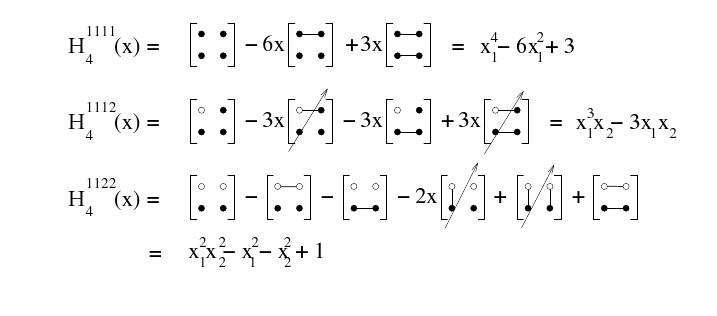
\includegraphics[width=7cm]{./Fig1.pdf}
  \end{center}
\caption{ Graphical representation of $H_4(x)$ tensor elements in two dimensions.}
\label{Fig1}
\end{figure}

The inclusion of mode-coupling necessitates consideration of mixed
indices (nondiagonal tensor elements). Here, we focus on the coupling
between mode pairs and ignore threesome and higher order mixing, i.e.,
we consider only the bi-polynomials ${\bf H}^{i_1i_2\dots
  i_\nu}_\nu(\Delta r_k,\Delta r_l)$ with $i_m \in \{k,l\}$,
$k,l=1,2,\dots,3N$. At first sight, estimating the contribution of
mode-coupling even at this lowest level appears to be a formidable
task, because for the optimal cut-off rank $\nu=16$ (see below), the
number of distinct expectation values to be extracted from the data
grows combinatorially. We show below that, the factorization property
of the off-diagonal tensor elements and the orthogonality of the modes
at the second order bring a significant reduction in complexity, which
we exploit to investigate the impact of anharmonicity and
mode-coupling separately on the protein dynamics.

In order to reach the desired formulation, we first note that the value
of a tensor element ${\bf H}^{i_1i_2\dots i_\nu}_\nu({\bf \Delta r})$
does not depend on the order of the indices due to the commutativity
of the gradient operator, $\nabla_i\nabla_j -
\nabla_j\nabla_i=0$. Therefore,
\begin{eqnarray}
{\bf H}^{i_1i_2\dots i_\nu}_\nu({\bf \Delta r}) &=& {\bf H}^p_\nu(\Delta r_k,\Delta r_l) \nonumber \\
\end{eqnarray}
where $p$ is the number of indices equal to $k$ (and the remaining
$\nu-p$ indices are equal to $l$). The fact that the covariance matrix
in $\{\Delta r\}$ basis is diagonal further implies that
\begin{eqnarray}
\label{factorization}
{\bf H}^{p,q}({\bf x}) &=& H_p(x_1)\times H_q(x_2)
\end{eqnarray}
as is evident from the Rodrigues's formula in Eq.(\ref{Rodrigues}).

Combining Eqs.(\ref{coefs})\&(\ref{factorization}), the Hermite
expansion in Eq.(\ref{hermite_expansion}) can be cast into the
following form:
\begin{widetext}
\begin{eqnarray}
\label{hermite_expansion2}
f({\bf\Delta r}) &=& \frac{1}{\sqrt{(2\pi)^N}} e^{ -\sum_i \Delta
  r_i^2/2} \bigg[ 1 + \sum_i\sum_{\nu=3}^\infty
  \frac{1}{\nu!}\, \Big\langle
  H_\nu(\Delta r_i)\Big\rangle\,H_\nu(\Delta r_i) \nonumber \\
&+&  \sum_{i\ne j}\sum_{\nu=3}^\infty
  \frac{1}{\nu!}\,\sum_{p=1}^{\nu-1} {\nu\choose p} \Big\langle
  H_p(\Delta r_i)H_{\nu-p}(\Delta r_j)\Big\rangle\,H_p(\Delta r_i)H_{\nu-p}(\Delta r_j) + \sum_{i\ne j\ne k} \cdots \bigg]
\end{eqnarray}
\end{widetext}
The first term in $[\cdots]$ corresponds to a purely harmonic
model. The next term is appriciable when the modes are anharmonic, but
gives no information about mode-coupling. In fact, the most general
mode-amplitude distribution of an anharmonic model composed of
decoupled modes is
\begin{eqnarray}
\label{decoupled}
f({\bf\Delta r}) &=& \frac{1}{\sqrt{(2\pi)^N}} e^{ -\sum_i \Delta
  r_i^2/2}\times \nonumber \\ && \prod_i \bigg[ 1 + \sum_{\nu=3}^\infty
  \frac{1}{\nu!}\, \Big\langle
  H_\nu(\Delta r_i)\Big\rangle\,H_\nu(\Delta r_i)\bigg]
\end{eqnarray}
The difference between Eq.(\ref{hermite_expansion2}) and
Eq.(\ref{decoupled}) is the mode-coupling corrections such as
\begin{eqnarray}
\langle H_p(\Delta r_i)H_{\nu-p}(\Delta r_j)\rangle - \langle
H_p(\Delta r_i)\rangle\langle H_{\nu-p}(\Delta r_j)\rangle &\neq& 0 \nonumber
\end{eqnarray}
and higher order cumulants. Note that, these corrections are transparent to the
marginal distributions
\begin{eqnarray}
\label{marginal}
f(\Delta r_i) &\equiv& \int_0^\infty \prod_{j\ne i}d\Delta r_j\ f({\bf\Delta r})\ 
\end{eqnarray}
as a merit of the orthogonality relation in
Eq.(\ref{orthogonality}). Therefore, even if the marginal
distributions are reproduced to good accuracy, the multi-dimensional
free-energy landscape of the protein may be very different from that
implied by a model based on Eq.(\ref{decoupled}). We demonstrate below
that this is the case for the protein ..

\begin{thebibliography}{99}

\bibitem{ENM}{ Reference GNM, ENM, etc.}
\bibitem{Yogurtcu}{ Yogurtcu {\it et al.} (2009).}
%% \bibitem{FPU}{Scholarpedia 3 (8) 5538 (2008) - Dauxois T and Ruffo S ``FPU nonlinear lattice
%% oscillations''}
\bibitem{mode_coupling_ref}{ Reference on mode coupling, enegry transfer between modes, etc.}
\bibitem{Flory}{Flory, 1976.}

\end{thebibliography}

\end{document}
